\documentclass{article}
\usepackage[english]{babel}
\usepackage[round,authoryear]{natbib}
\usepackage{graphicx}
\usepackage{amsmath}
\bibliographystyle{abbrvnat}

\title{\textbf{MOCCA} \\
\large Multi-sourced Oceanic Carbonate Chemistry Assimilation}
% maybe also \title{Uncertainties from deep learning in climate science}
% maybe also robustness
% maybe also: Traceability
% Or; epistemic implications of deep learning in cliamte science
% https://www.frontiersin.org/articles/10.3389/frai.2023.974295/full
% https://www.nature.com/articles/s42256-022-00592-3
% https://christophm.github.io/interpretable-ml-book/neural-networks.html
% https://ieeexplore.ieee.org/document/9521221
% https://towardsdatascience.com/dense-or-convolutional-part-2-interpretability-c310a9fd99a5 (only image classification)
% https://en.m.wikipedia.org/wiki/Universal_approximation_theorem
%https://www.scribd.com/document/468040826/Approximation-with-Artificial-Neural-Network-MSc-Thesis-2001-pdf
%https://deeplearningdiary.com/2023/11/26/universal-approximation-theorem-the-infinitely-squiggly-function/
%https://medium.com/analytics-vidhya/you-dont-understand-neural-networks-until-you-understand-the-universal-approximation-theorem-85b3e7677126
%https://ai.stackexchange.com/questions/17670/how-can-supervised-learning-be-viewed-as-a-conditional-probability-of-the-labels
%https://towardsdatascience.com/understanding-objective-functions-in-neural-networks-d217cb068138

% alternatives
% \title{When are machine learning based predictions in climate science accurate?}
% \title{Interpretability of neural-network-based results in climate science?}
% \title{What can be learned from machine learning models in climate science?}
\author{Friedrich Burger}
\date {February 2024}

\begin{document}
	
	\maketitle
	\tableofcontents
	\section{Introduction}
	neural networks...\cite{goodfellow2016}
	\section{Model architecture}
	\subsection{Overview}
	\begin{figure}
		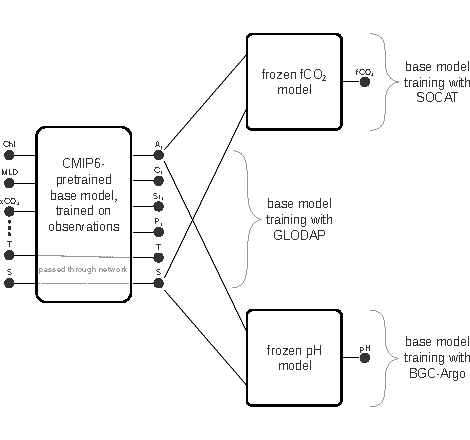
\includegraphics[width=0.85\textwidth]{./figures/model_architecture_scheme.pdf}
		\caption{Scheme displaying the overall model architecture of MOCCA.}
		\label{fig:fco2_model}
	\end{figure}
	\subsection{Surrogate models for mocsy fCO2 and pH}
	In a first step, surrogate multi-layer perceptron models were trained to replace numerical solution of the oceanic carbonate system. To do so, samples for total alkalinity (A$_\textup{T}$), dissolved inorganic carbon (C$_\textup{T}$), temperature (T),  salinity (S), total silicate (Si$_\textup{T}$), and total phosphate (P$_\textup{T}$) were randomly generated from uniform distributions (Table~\ref{tab:gen_data}). \\
	The training data size was set to 5 000 000 samples and the validation data size was set to 1 000 000 samples. Mocsy 2.0 (Orr et al., 2015a) was then used to calculate fCO$_2$ and pH for these samples. After normalizing per feature with the means and standard deviations given in Table~\ref{tab:gen_data}, multilayer perceptron models with three identical hidden layers were trained with mocsy fCO$_2$ and pH as labels. \\
	For fCO$_2$, model complexity was iteratively increased until a desired maximum deviation of less than 1\,$\mu$atm was reached (the measurement uncertainty for pCO$_2$ as reported by Orr et al, 2015b)\footnote{For reference, fCO$_2$ across the generated samples varies between 8\,$\mu$atm and 4317\,$\mu$atm.}. During training, batch size was iteratively increased from 1000 to 500 000 and learning rate was iteratively decreased from 10$^{-3}$ to 10$^{-5}$ over up to 10 000 epochs. The increase in batch size and decrease in learning rate was implemented to shift from an initial identification of an optimal region in the parameter space to finding an optimal set of parameters for which the mean squared error over the training and validation sets converges to a similar and low value. \\
	Hidden layer size was increased from an initial 64 hidden layer units (8833 trainable parameters), 80 units (13601 parameters), 96 units (19393 parameters), 128 units (34049 parameters), to 160 units (52801 parameters). The largest model\footnote{To give some context about the model complexity: The number of paramters of this model is comparable to that of a Taylor expansion of a function with six arguments to 15th order. Assuming an efficient use of the MLP parameters, a good fit to the numerical solution from mocsy is thus expected.} hit a maximum deviation of 0.87\,$\mu$atm over the validation set (Figure~\ref{fig:fco2_model}).
	The same model architecture was then also used to train the pH model, %albeit with longer training time (14 000 epochs instead of 10 000 for the fCO$_2$ model, extendind the last training step with a learning rate of 10$^{-5}$ to enable convergence on both the training and validation sets), 
	resulting in a maximum deviation over the validation set of 0.0023. \\
	With root mean squared deviations of 0.034\,$\mu$atm (fCO$_2$ model) and 0.00006 (pH model), these surrogate models provide a precision that is comparable to numerical carbonate chemistry packages: Orr et al., 2015b report a desired numerical uncertainty of 0.1\,$\mu$atm and 0.0003, respectively.
	
	\begin{table}
		\centering
		\bgroup
		\def\arraystretch{1.5}
		\begin{tabular}{c|c|c}
			& minimum & maximum \\
			\hline 
			A$_\textup{T}$ & 1700\,$\mu$mol\,kg$^{-1}$ & 2700\,$\mu$mol\,kg$^{-1}$ \\
			\hline
			C$_\textup{T}$ & 1700\,$\mu$mol\,kg$^{-1}$ & A$_\textup{T}$ \\
			\hline
			T & 2\,°C & 35\,°C \\
			\hline
			S & 19\,PSU & 43\,PSU \\
			\hline
			Si$_\textup{T}$ & 0\,$\mu$mol\,kg$^{-1}$ & 134\,$\mu$mol\,kg$^{-1}$ \\
			\hline
			P$_\textup{T}$ & 0\,$\mu$mol\,kg$^{-1}$ & 4\,$\mu$mol\,kg$^{-1}$ \\
			
		\end{tabular}
		\egroup
		\caption{Minima and maxima of the uniform distributions used to generate samples for the fCO$_2$ and pH surrogate models. The range for A$_\textup{T}$ was chosen such that it easily encompasses open ocean variations in A$_\textup{T}$. That for C$_\textup{T}$ is limited to values lower A$_\textup{T}$ since larger C$_\textup{T}$ do not occur in the ocean. The ranges for T and S are chosen according to Lueker et al., 2000, whose parameterizations for K$_1$ and K$_2$ are used in mocsy. Finally, the maximum values for Si$_\textup{T}$ and P$_\textup{T}$ were chosen to be the global maxima found in the monthly climatologies for Si$_\textup{T}$ and P$_\textup{T}$ from World Ocean Atlas 2023. These uniform distributions have means $(max + min) / 2$ and standard deviations $(max - min) / \sqrt{12}$, expcept for C$_\textup{T}$ where mean and standard deviation are given by $min + (max - min) / 4$ and $(max - min) \cdot \sqrt{7 / 144}$, respectively. These means and standard deviations are used for feature normalization.}
		\label{tab:gen_data}
	\end{table}
	\begin{figure}
		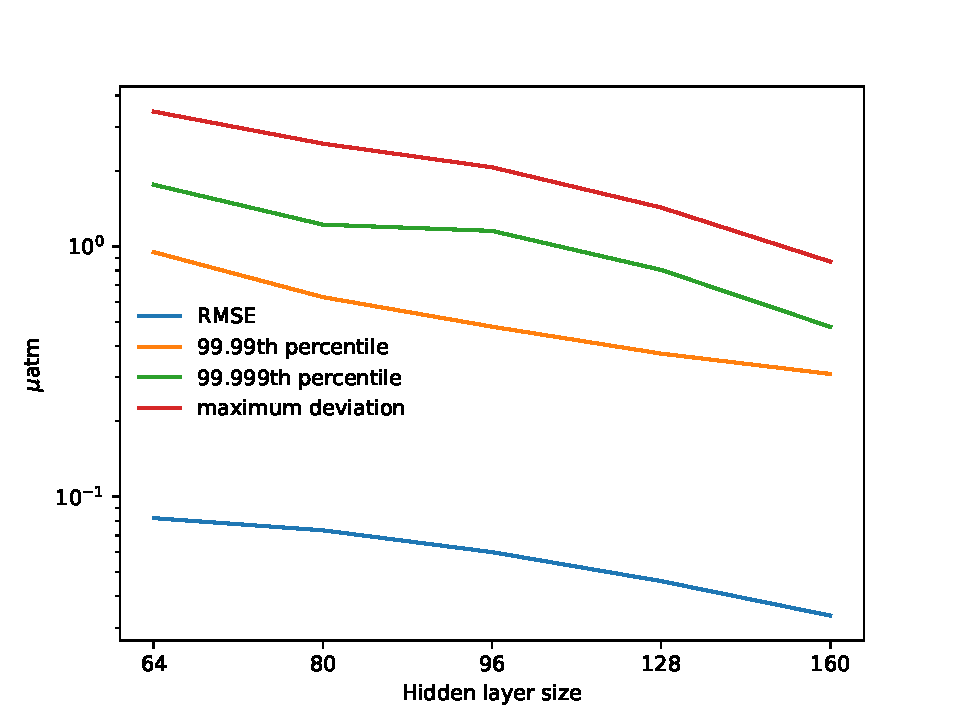
\includegraphics[width=0.85\textwidth]{./figures/fco2_model_error_vs_hidden_layer_size.pdf}
		\caption{The evolution of root mean squared error (RMSE), the 99.99th and 99.999th percentiles of deviation and the maximum deviation between the surrogate model and mocsy fCO$_2$ over the validation data set with 1000 000 randomly generated samples.}
		\label{fig:fco2_model}
	\end{figure}
	\subsection{CMIP6-pretrained DIC and Alk model}
	\subsection{SOCAT-, GLODAP-, and BGC-Argo-based model tuning}
	\section{Model performance}
	\medskip
	
	\bibliography{bib}
	
\end{document}